\chapter{Overview of the $\text{M}_\text{T2}$ Analysis}

\section{Motivation for an all-hadronic search}

\begin{figure}[h]
  \begin{center}
    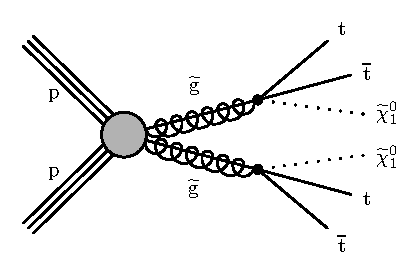
\includegraphics[width=0.40\textwidth]{figs/susy_diagrams/T1tttt.pdf}
    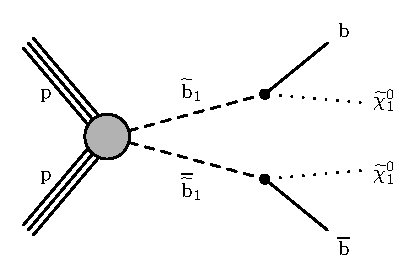
\includegraphics[width=0.40\textwidth]{figs/susy_diagrams/T2bb.pdf}
    \caption{Example Feynman diagrams of strongly-produced SUSY particles decaying hadronically.
      (left) Gluino pair production, where each gluino decays into a neutralino and two top quarks.
      (right) Bottom squark pair production, where each squark decays into a neutralino and bottom quark.
            }
    \label{Fig:example_susy_feyn}
  \end{center}
\end{figure}


\section{The $M_\text{T2}$ variable}
\newcommand{\ptvis}{\ensuremath{\pt^\mrm{vis}}\xspace}
\newcommand{\vptvis}{\ensuremath{\vec{p}_{\> \mathrm{T}}^{\> \mathrm{vis}}}\xspace}

Defining the \emph{transverse energy} of a particle as $E_\mrm{T}^2\equiv m^2+\pt^2$, we can define the \emph{transverse mass} of a two-particle system as
\be
\begin{split}
M_\mrm{T}^2 &\equiv (E_\mrm{T,1}+E_\mrm{T,2})^2 - (\vec{p}_\mrm{T,1} + \vec{p}_\mrm{T,2})^2 \\
&= m_1^2 + m_2^2 + 2(E_\mrm{T,1}E_\mrm{T,2} - \vec{p}_\mrm{T,1}\cdot\vec{p}_\mrm{T,2}).
\end{split}
\ee

Assuming massless particles (or, equivalently, that they are highly relativistic such that $E\gg m$ and $E_\mrm{T}\approx\pt$), this simplifies to
\be\label{eq:mt}
M_\mrm{T}^2 = 2p_\mrm{T,1}p_\mrm{T,2}(1-\cos\theta),
\ee
where $\theta$ is the opening angle between the particle momentum vectors.

This variable is frequently useful when a particle decays to something visible and something invisible (e.g. $W\to e\nu$).
Assuming that the invisible particle is the dominant source of missing energy in the event, the \vMet vector is approximately the
transverse momentum vector of the invisible particle and can be plugged into Eq.~\ref{eq:mt} to compute the transverse mass of the
system. As the transverse mass is just the invariant mass computed only with the transverse components of the particle momenta,
it naturally has an upper bound equal to the parent particle mass. An example from a CMS measurement of the $W$ production
cross section \cite{CMS:w_prod} is shown in Fig.~\ref{Fig:w_transverse_mass}. In this case, the two-particle system is
$W\to\mu\nu$ decay, and $M_\mrm{T}\lessapprox M_W=80~\GeV$. The small number of events with transverse mass larger than the $W$ mass
are due to experimental resolution on the muon momentum and \vMet vectors.

\begin{figure}[t]
  \begin{center}
    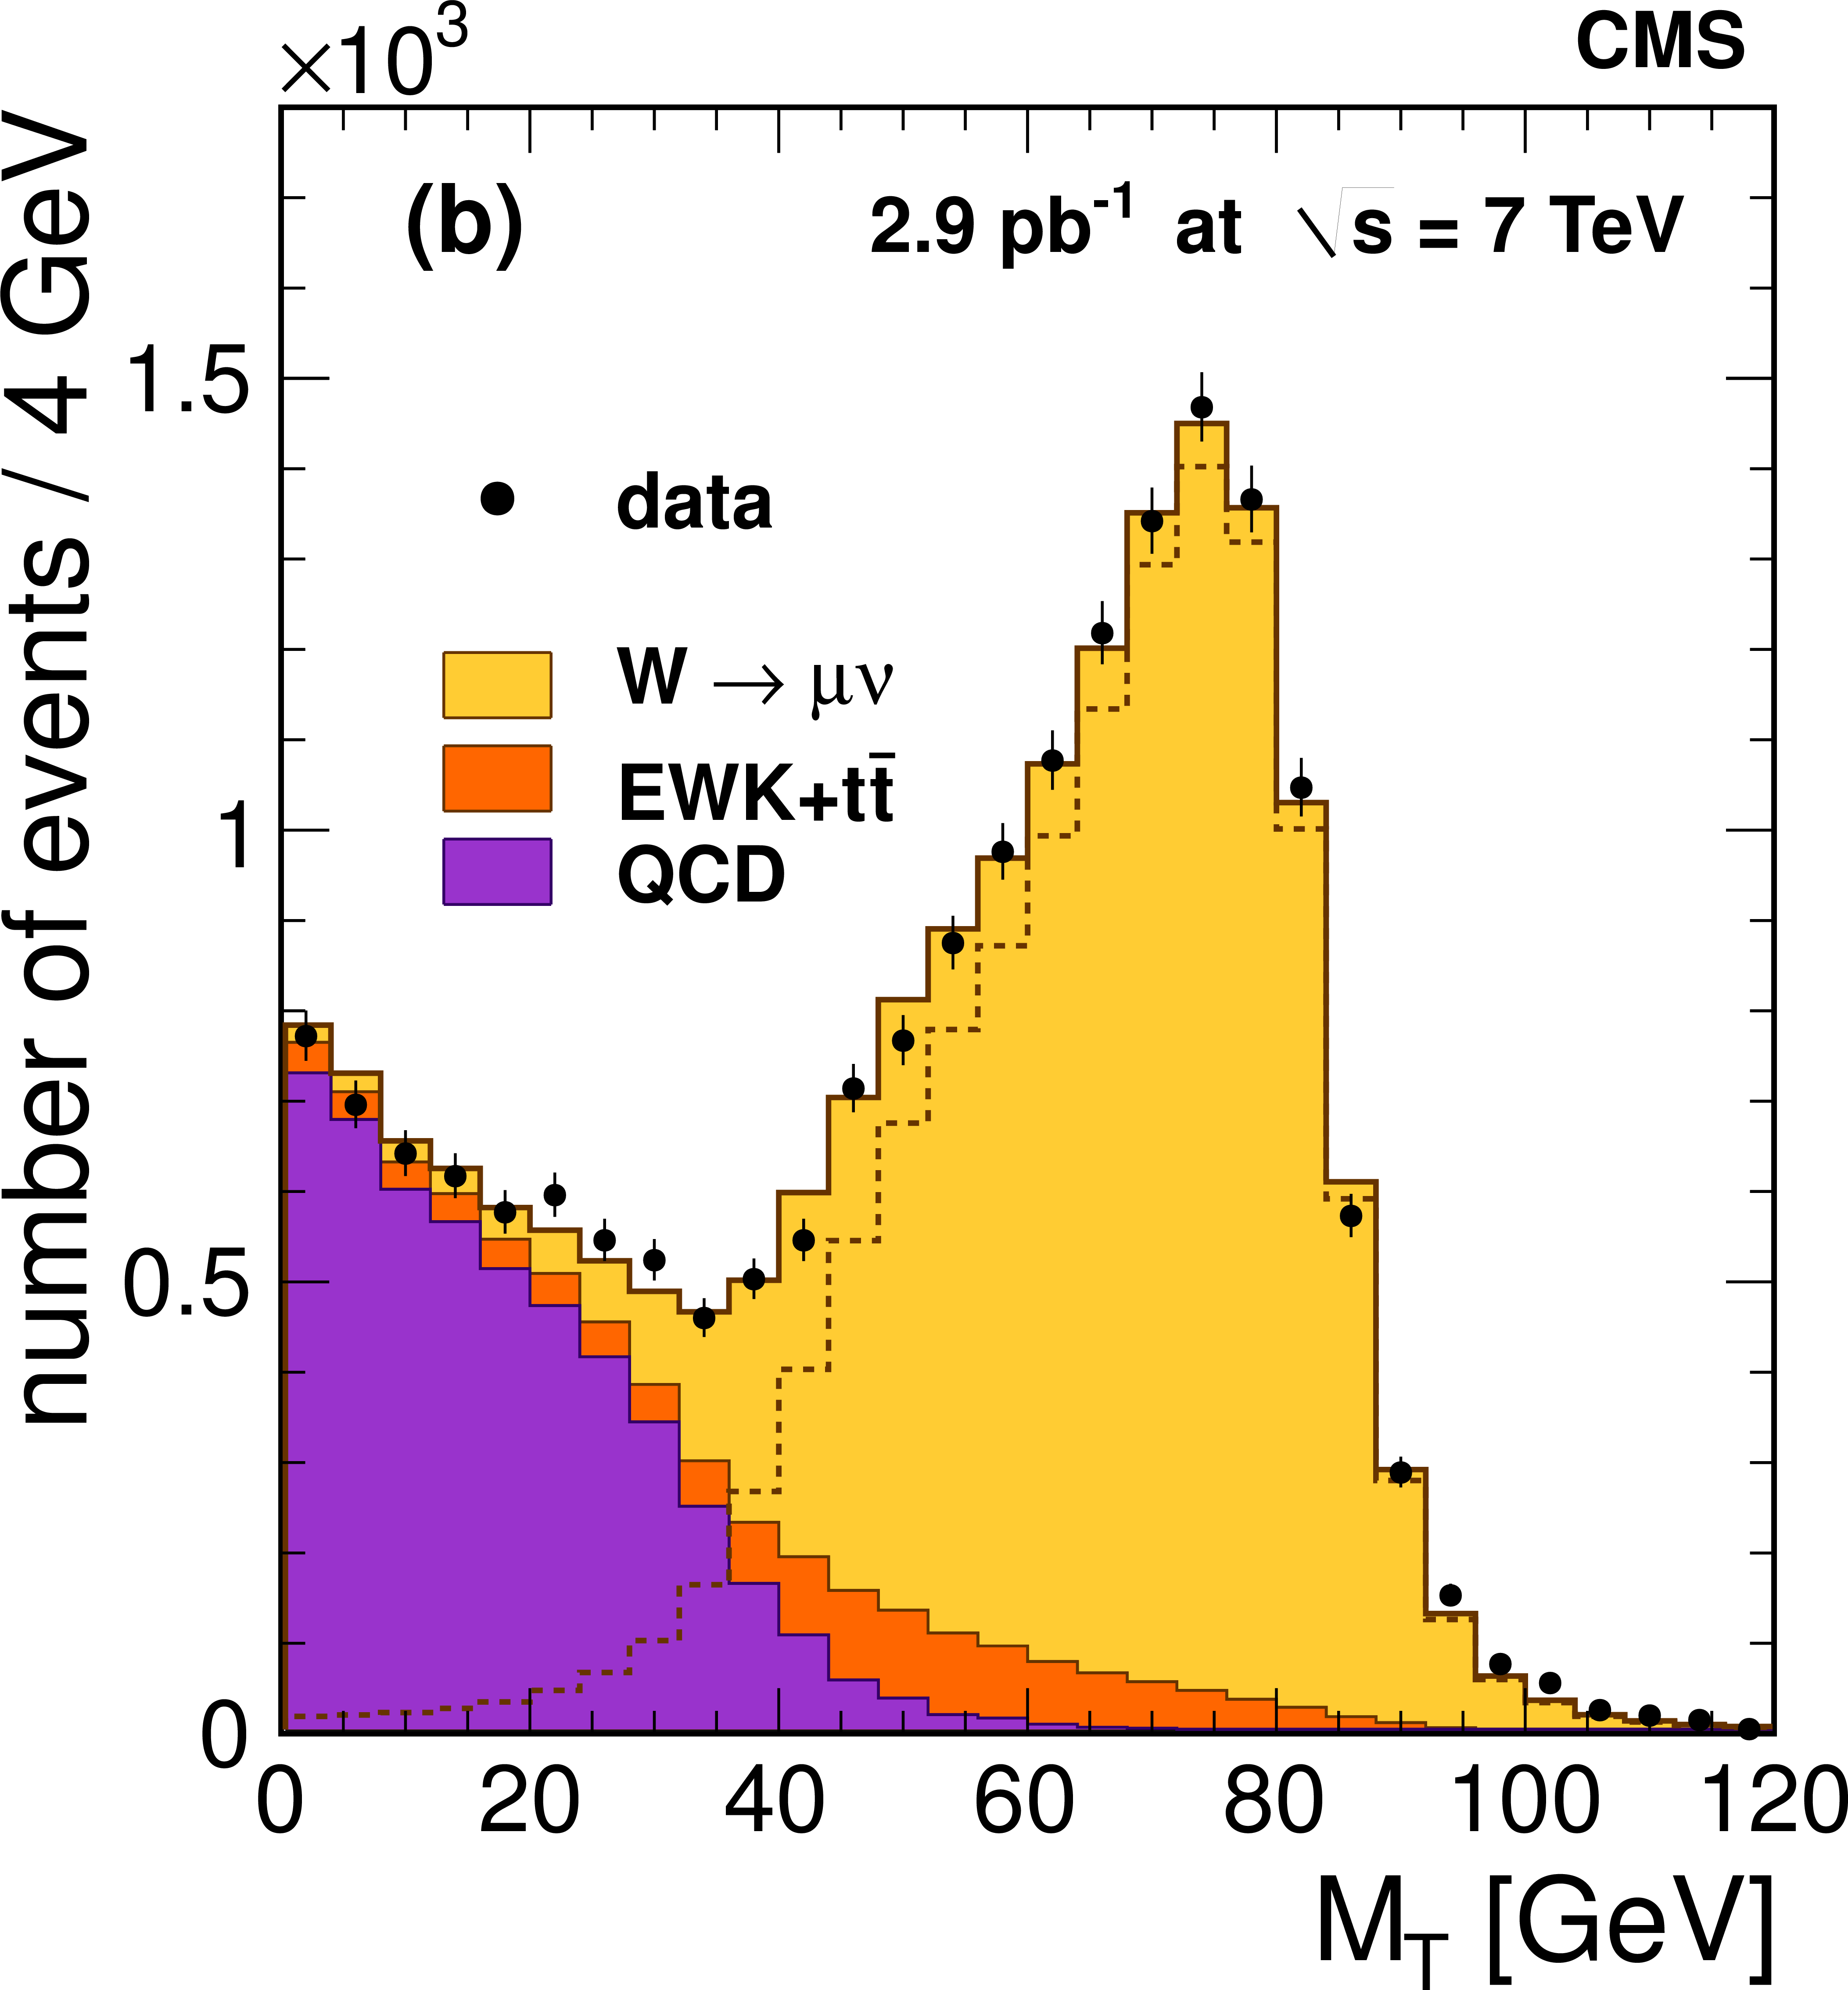
\includegraphics[width=0.45\textwidth]{figs/overview_mt2/w_transverse_mass.png}
    \caption{Transverse mass of the muon-\vMet system from a CMS measurement of the $W$ production cross section \cite{CMS:w_prod}.
      The transverse mass has a rough upper bound at $M_W=80~\GeV$, limited by experimental resolution.
            }
    \label{Fig:w_transverse_mass}
  \end{center}
\end{figure}



\section{Sources of backgrounds}
